\section{Methodology}

\subsection{Datasets}

\subsubsection{AI-ELT}

Our in-house dataset was collected on 11-12th October 2023 at the 8th Urology Boot Camp in Leeds, United Kingdom \cite{urology2023}. It contains 24 videos, each a trial performed by a single participant. All participants, surgical trainees and trainers were given a handout, as shown in Figure \ref{fig:dataset-collection}, which explained the study and the data collection process. We used a Simulated Insufflated Belly Laparoscopic Trainer Simulator Training Box with 30 Degree 1920x1080 HD Camera \cite{aliexpress}. The sensors were three NDI Aurora 6DoF (Six Degrees-of-Freedom) electromagnetic trackers (one on each tool and one on the camera) \cite{hummel_design_2005}. The calibrated position was to the fulcrum of each tool, performed by pivot calibration (see the black reference point on the right of the peg transfer board with the blue tape in Figure \ref{fig:test1_issues}). Handedness data was collected using the Edinburgh Handedness survey in various other tasks, including main hand for writing, drawing, throwing, using scissors, toothbrush, etc. \cite{oldfield_assessment_1971}. Level of expertise was estimated using the number of procedures in their lifetimes and within the last 12 months. Participants were confirmed not to have a pacemaker or other metal implants which could interfere with the electromagnetic tracking system. In this study, there was no need for any participant follow-up.

% Generally compared to other datasets, the camera was of higher resolution with increased field-of-vision (FOV), contained two tools in all procedures (many laparoscopic videos contain just a single tool), and 6DoF ground truth three-dimensional tooltip positions and spatial rotation quaternions. Surgeon information included data about the participants' handedness and level of expertise.

\begin{figure}[tbp]
    \centering
    \vspace*{-2.5mm}
    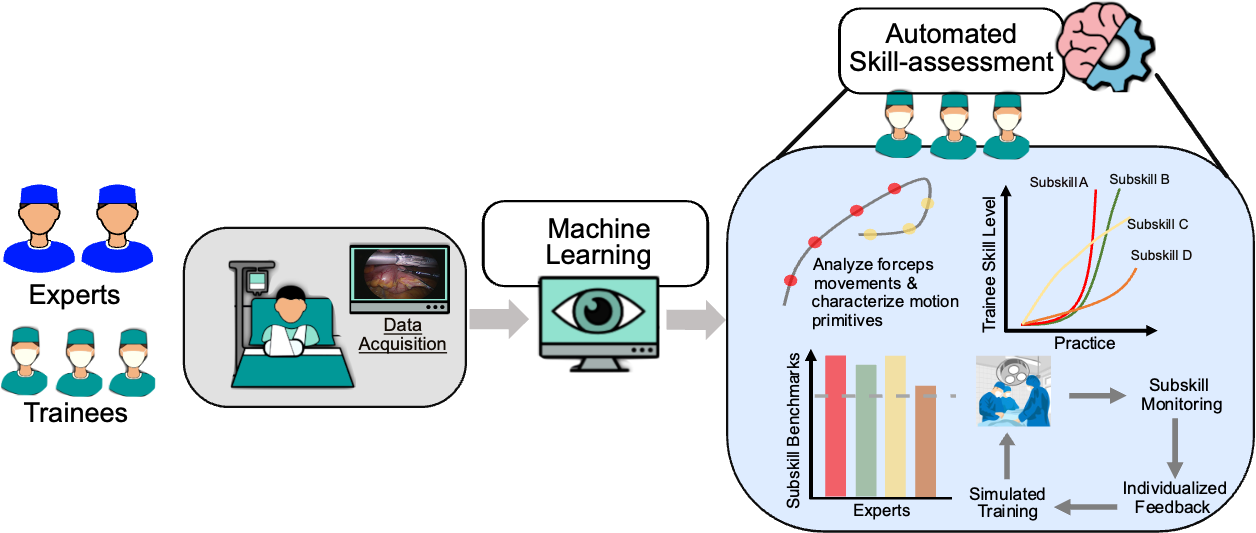
\includegraphics[width=1\linewidth]{dataset_collection.png}
    \vspace*{-6.5mm}
    \caption{AI-ELT Dataset Collection}
    \vspace*{-3mm}
    \label{fig:dataset-collection}
    \Description{Handout given to surgeons preceding the data collection process.}
\end{figure}

%% The handout explained that the study was to collect motion data from a peg transfer task. The goal was to train an AI system to localise the laparoscopic tools using the image alone. This would help develop a new training system, giving automated feedback on individual sub-skills. In this study, we focused on first detecting the tools, which could then be used with the sensor data to build a model which could predict the tools' motion based on the tool's location in the image.

The final dataset comprises 24 laparoscopic surgery videos, each approximately 3 minutes long in 1920x1080 resolution, totalling 1.32GB of 103,629 frames annotated with the 6DoF ground truth data. The first trial contained extra lighting causing visual defects (see Figure \ref{fig:test1_issues}), which was removed for subsequent trials.

\begin{figure}[htbp]
    \centering
    \vspace{-2.5mm}
    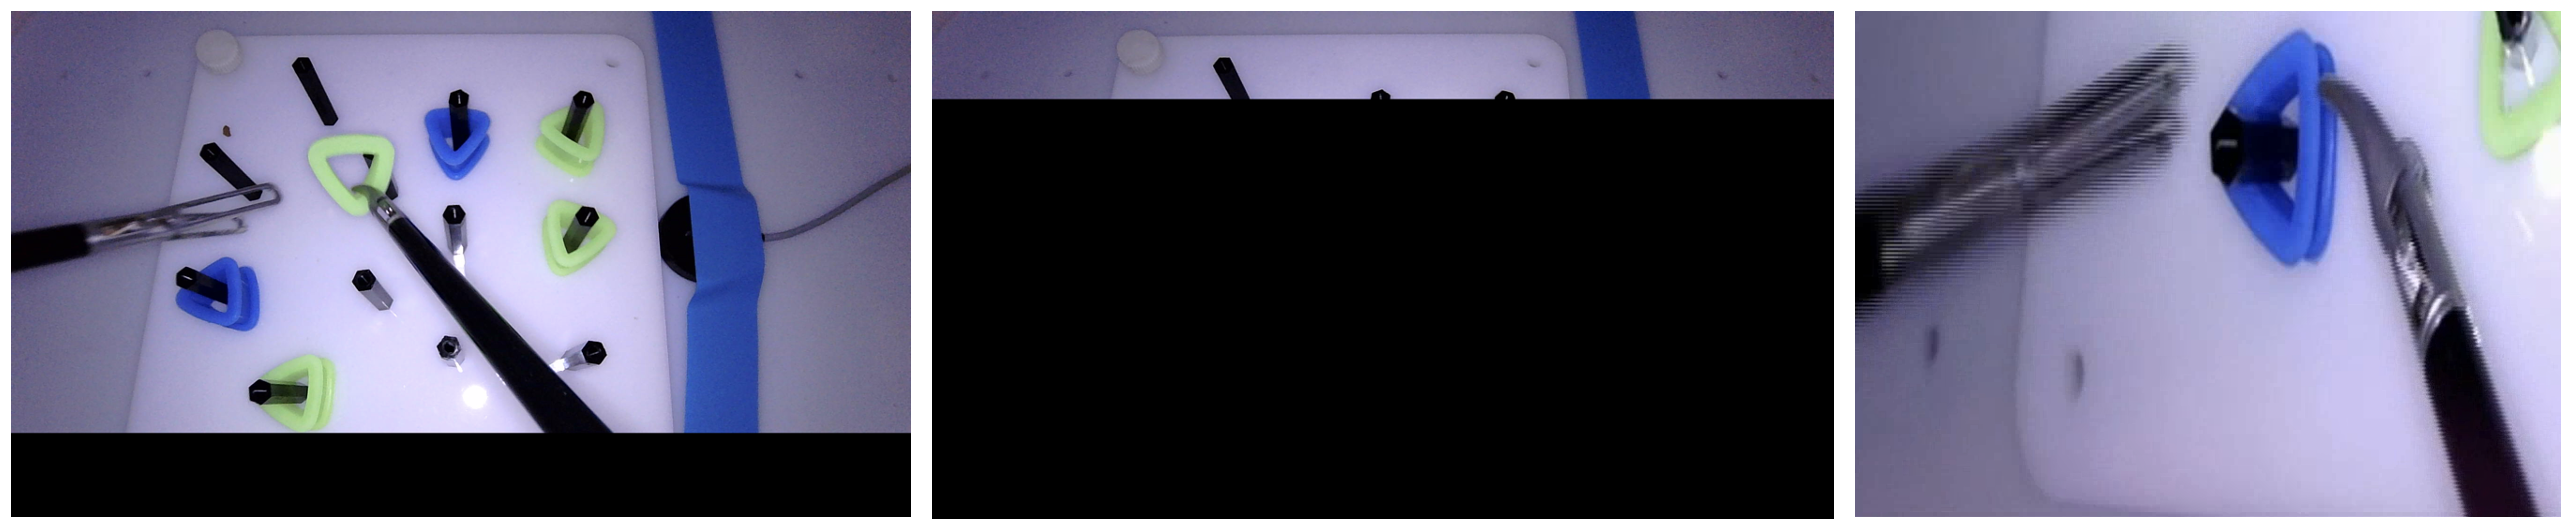
\includegraphics[width=1\linewidth]{test1_issues}
    \vspace*{-7.5mm}
    \caption{Issues with the dataset}
    \vspace*{-5mm}
    \label{fig:test1_issues}
    \Description{We see a few issues with the dataset. Of all 24 videos, 1 emits extra light onto the scene (Test 1). We also see some frames have been cut off, either a little (\textit{left}) or a lot (\textit{middle}). We also note some camera overheating, causing image defects (\textit{right}).}
\end{figure}

% The average number of procedures performed was 120, with a range of 0 to over 1000, with 22 estimated to be performed on average in the last 12 months, ranging from 0 to 100. All 24 participants agreed to share their results entirely. If we categorise the surgeon's skills based on several procedures, where low is <20, medium is between 20 and 100, and high is >100, then we have 9 low, 9 medium and 6 high-skilled surgeons. Results from the Edinburgh Handedness survey \cite{oldfield_assessment_1971} showed almost all surgeons were right-handed, with one left (participant 12) and one who alternated hands (participant 3).

% The results of the Edinburgh Handedness survey \cite{oldfield_assessment_1971} could be used to evaluate surgical skills based on the handedness of the surgeon. Further annotations could be developed based on existing metrics of technical surgeons, e.g. Objective Structured Assessment of Technical Skills (OSATS) \cite{martin_objective_1997, hussein_development_2017}. Though based on questionnaires and subjective, they could help set a baseline for categorising surgical skill level \cite{hilal_randomized_2017}. Key movement metrics which define the skill level for typical tasks in a laparoscopic procedure can be identified \cite{pears_capturing_2021}. These metrics can be quantified from trainee videos to create task-specific learning curves.

\subsubsection{Data Preparation}

To ensure robust model validation, we have manually labelled 1\% of the images across 23 videos and one video fully labelled as a test set (Video 5) by modifying an existing keypoint annotation tool \cite{herrera_luiscarlosgphkeypoint-annotation-tool_2024}. Annotations were recorded in a text file in Common Object in Context (COCO) format with class (either tool or tooltip), bounding box centre ($x$), bounding box centre ($y$), width and height. Values were normalised to the size of the image to allow better generalisability. No duplicates, outliers or inconsistencies were noticed. However, we see a few issues with the dataset (Figure \ref{fig:test1_issues}). Some frames have been cut off, either a little (\textit{left}) or a lot (\textit{middle}). We also note some camera overheating, causing image defects (\textit{right}). We appropriately removed missing data for model training, giving 864 clean training data files out of 1045.

Our code contains multiple helper functions and classes to assist in future development \cite{choudhry_omarioscmsc-surgical-tool-tracking_2024}. This will be adapted to a more formal AI-ELT framework in the future. Before manual annotation, we attempted to get the objects' $x$ and $y$ positions using ground truth 3D position data, matrix transformations with intrinsic and extrinsic camera and scene parameters, and regular linear regression. However, the error margin was too high. The best-produced model could be used to annotate remaining bounding boxes with weak labels in a teacher-student framework or for a more complex model to reverse-engineer positions from motion data in future datasets \cite{teevno_semi-supervised_2023}. Inspired by the CholecTrack20 schematic diagram, we present an intuitive way to understand the dataset \cite{nwoye_cholectrack20_2023}.

\begin{figure}[htbp]
    \centering
    \vspace*{-2mm}
    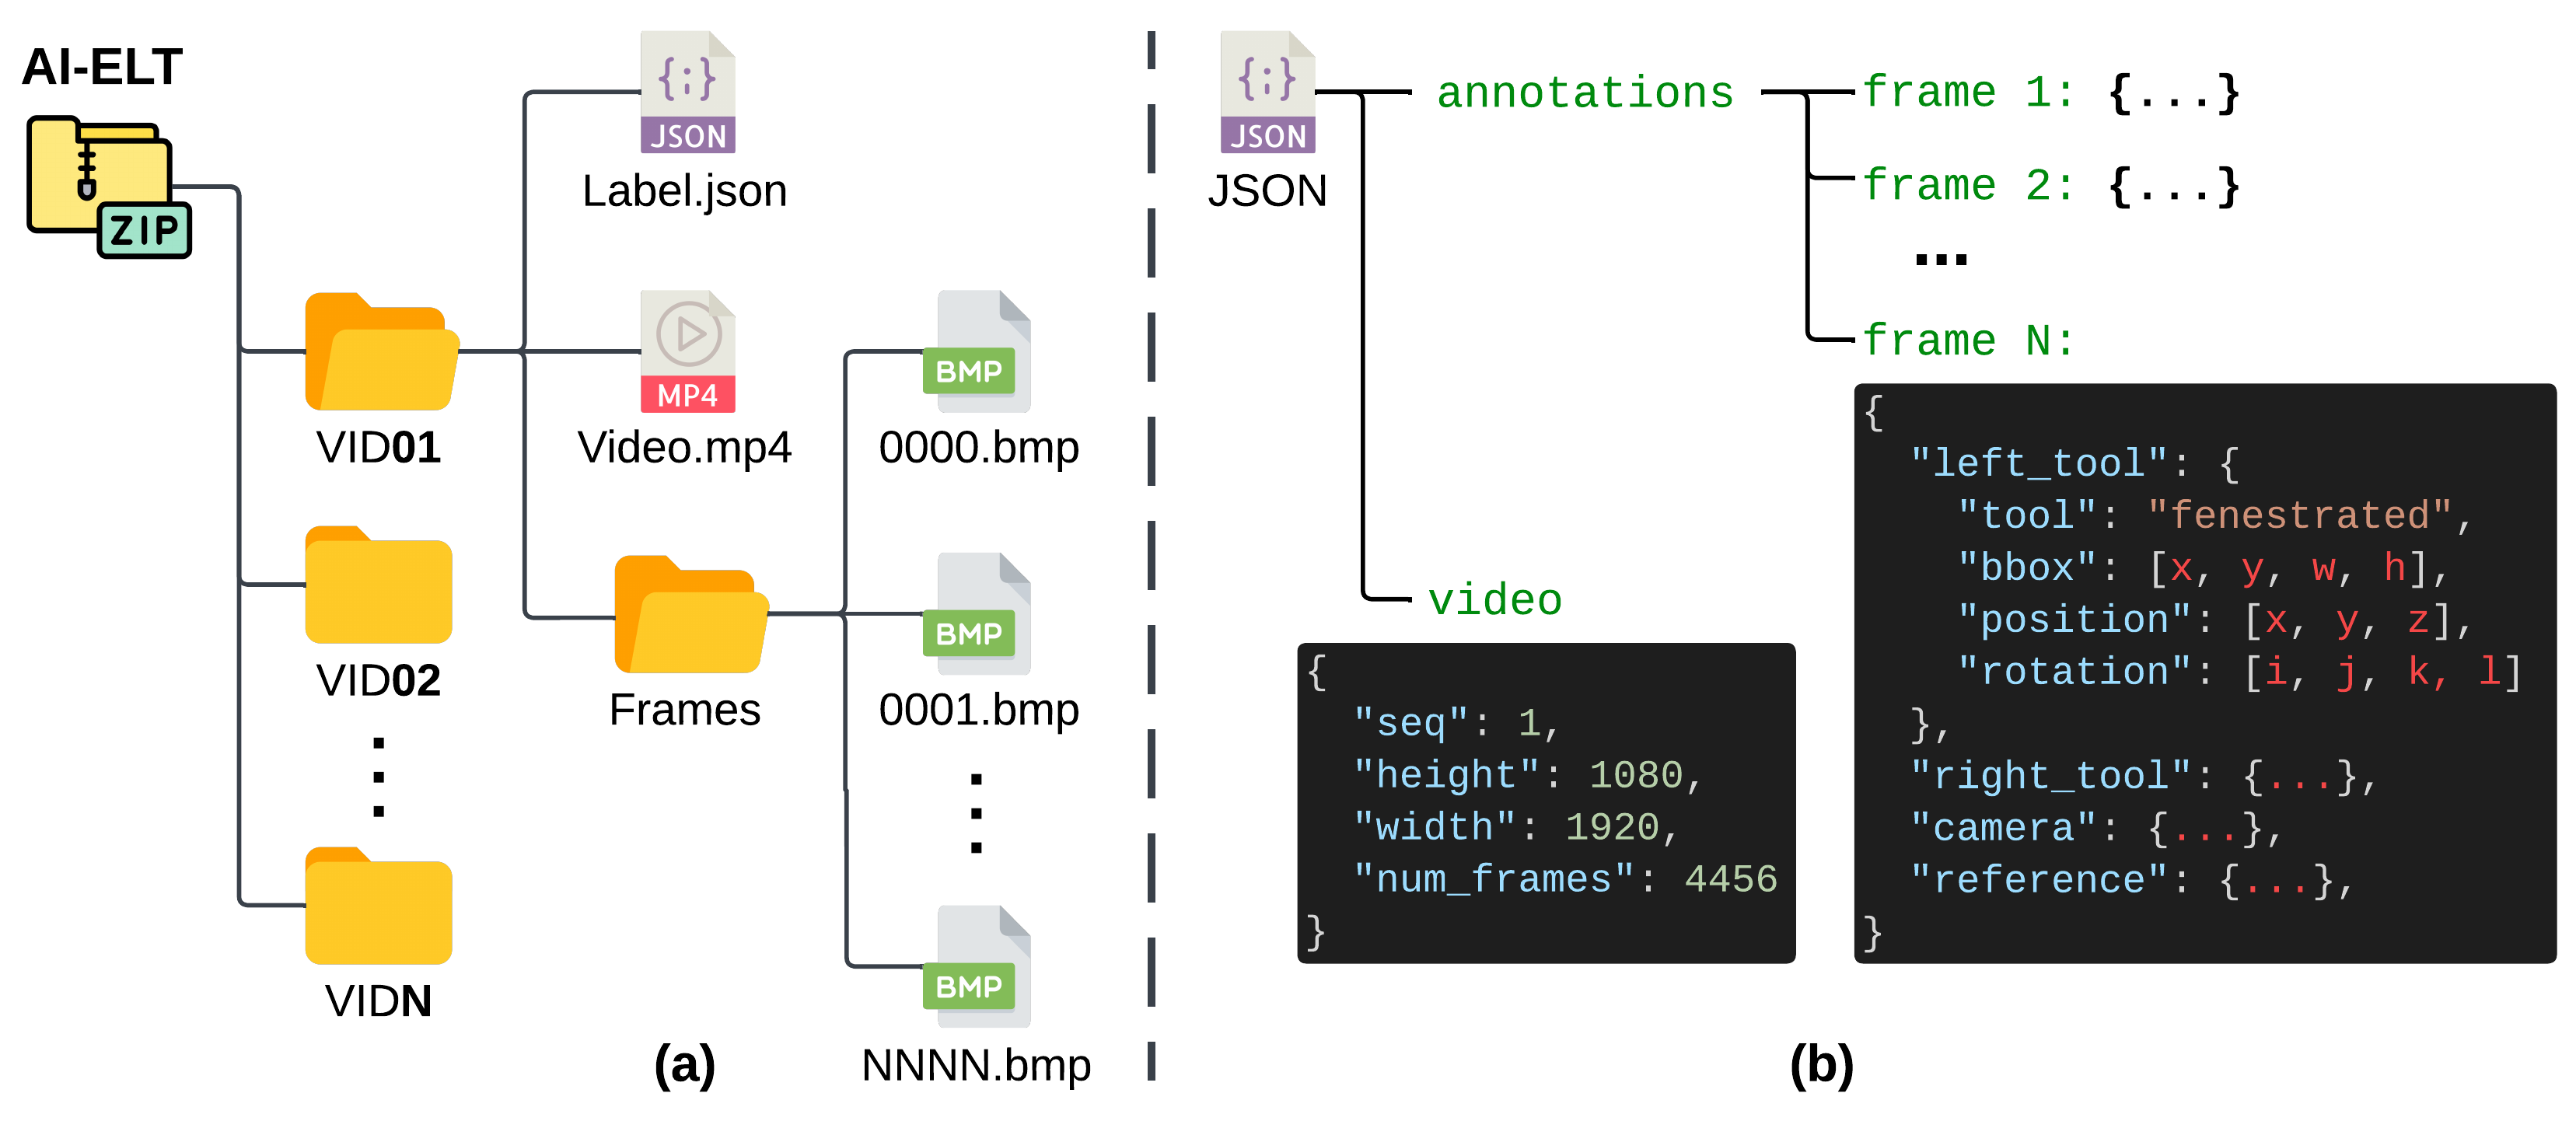
\includegraphics[width=\linewidth]{schematic_diagram.png}
    \vspace*{-7.5mm}
    \caption{Schematic diagram of the dataset files showing (a) folder structure for the dataset and (b) Data structure for the JSON label files.}
    \vspace*{-5mm}
    \label{fig:schematic_diagram}
    \Description{Schematic diagram for the AI-ELT Dataset}
\end{figure}

\subsubsection{Other Datasets}

The final decision was to perform additional extensive evaluation solely on the ART-Net dataset \cite{hasan_detection_2021}. Since we will re-implement the ART-Net model (with its code already available), it is logical to use the same dataset to evaluate the reproducibility and a more objective evaluation of the methods by comparing results. We converted the ART-Net tool and tooltip segmentation maps to bounding boxes (1,324 training images and 308 test images). We will keep the dataset's negative examples, which do not contain any tools to attempt to reduce potential false positives.

\subsection{Reimplementation of the State-of-the-Art}

Multiple anchor-based and anchor-free deep learning SOTA models are implemented and tested to consider LMIC resource constraints. The models were trained on a system with the following configuration: AMD Ryzen 3900X CPU, 32GB RAM, and an NVIDIA GeForce RTX 3060 GPU with 12GB of memory, running on Windows 11 Pro with Python 3.9.5 and PyTorch 2.2.1+cu121. In practice, the goal is to ensure these models can eventually be deployed on even less powerful and more affordable hardware. We use transfer learning by fine-tuning models with SOTA checkpoints to reduce training times and multiclass and multitask learning to meet our detection requirements \cite{alabi_multitask_2024}.

\subsubsection{Anchor-based Object Detection}

We tested all six different architectures of YOLOv10 (X, L, B, M, S, N) to investigate the effect of parameters and architecture size on inference and precision. RetinaNet and EfficientDet were trained with their default configurations. We also ran RetinaNet with anchor-box scale and ratio optimisation, which is expected to improve on results without anchor-box optimisation \cite{zlocha_improving_2019}.

\subsubsection{Anchor-free Object Detection}

The anchor-free models we tested were all five different architectures of YOLOv8 (X, L, M, S, N), the SIMO ART-Net model (with a ResNet 50 backbone for faster inference \cite{koonce_resnet_2021} and the original VGG 16 backbone \cite{hasan_detection_2021}) and the End-to-End DEtection TRansformer (DETR). The SIMO model was completely reimplemented from Tensorflow into PyTorch with a modified final layer to output bounding box annotations for left and right tools and tips. Without the segmentation information, we expect worse results than reported by Hasan \cite{hasan_detection_2021}. YOLOv8 and DETR were trained with their default configurations.

\subsubsection{Tracking Algorithm}

Though we discussed SOTA tracking algorithms, we can use a more efficient algorithm custom to our dataset and for similar contexts. We first identify each tool by checking the bottom half of its bounding box to determine the shaft axis direction — left tools exhibit a positive gradient, and right tools exhibit a negative gradient. Once a tool is identified, the tooltip detected within its bounding box inherits the tool's ID. A probabilistic model then uses previous predictions and the Euclidean distance between bounding box centres to inform decisions, ensuring consistent tracking and reidentification if a tool temporarily leaves the frame or is obscured. Without quantitative data for tracking, evaluation can be done qualitatively against ByteTrack \cite{ByteTrack} and Bot-SORT \cite{BoT-SORT} using the YOLO models. However, our algorithm should deal with issues in re-ID and be simpler and more efficient than methods such as SurgiTrack \cite{SurgiTrack}.

% Styles for the nodes and arrows
\tikzstyle{startstop} = [rectangle, rounded corners, minimum width=1cm, minimum height=0.3cm, text centered, draw=black, fill=red!30, font=\tiny]
\tikzstyle{process} = [rectangle, minimum width=0.7cm, minimum height=0.3cm, text centered, draw=black, fill=orange!30, font=\tiny]
\tikzstyle{decision} = [diamond, minimum width=0.5cm, minimum height=0.3cm, text centered, draw=black, fill=green!30, font=\tiny]
\tikzstyle{arrow} = [thick,->,>=stealth,font=\tiny]

%%%
% \begin{center}
% \begin{tikzpicture}[node distance=0.75cm]

% % Nodes
% \node (start) [startstop] {Start};
% \node (identify) [process, below of=start] {Identify Tool by Checking Bottom Half of Bounding Box};
% \node (gradient) [decision, below of=identify, yshift=-0.85cm] {Shaft Axis Direction?};
% \node (lefttool) [process, below of=gradient, xshift=-1.75cm, yshift=-0.25cm] {Left Tool};
% \node (righttool) [process, below of=gradient, xshift=1.75cm, yshift=-0.25cm] {Right Tool};
% \node (inheritID) [process, below of=gradient, yshift=-0.7cm] {Tooltip Inherits Tool's ID};
% \node (probModel) [process, below of=inheritID] {Use Probabilistic Model (Previous Predictions + Euclidean Distance)};
% \node (reidentify) [process, below of=probModel] {Reidentification if Tool is Obscured or Leaves Frame};
% \node (end) [startstop, below of=reidentify] {End};

% % Arrows
% \draw [arrow] (start) -- (identify);
% \draw [arrow] (identify) -- (gradient);
% \draw [arrow] (gradient) -- node[anchor=east] {Positive} (lefttool);
% \draw [arrow] (gradient) -- node[anchor=west] {Negative} (righttool);
% \draw [arrow] (lefttool) |- (inheritID);
% \draw [arrow] (righttool) |- (inheritID);
% \draw [arrow] (inheritID) -- (probModel);
% \draw [arrow] (probModel) -- (reidentify);
% \draw [arrow] (reidentify) -- (end);

% \end{tikzpicture}
% \end{center}

\subsubsection{Model Training}

The models were trained using default configurations, ensuring consistency across different architectures and datasets. Specific hyperparameters included a batch size of 16 (8 for memory-intensive models like SIMO and EfficientDet) and patience set to 10, allowing early stopping if validation performance did not improve after 10 epochs. Inference times were calculated based on the detection times per image over the test set. The YOLOv10 models trained on the AI-ELT dataset were fine-tuned versions of the models initially trained on the ART-Net dataset, which slightly reduced the iterations required for convergence. RetinaNet models with anchor-based optimisation were also fine-tuned versions of their non-optimised counterparts. Validation testing frequency was reduced to every 10 epochs to expedite training, especially for models with longer convergence times.

% YOLO models employed a specific type of mosaic augmentation to improve generalisation, where images are cropped and stitched together to form a larger image, increasing the model's robustness to different spatial contexts. 

\subsubsection{Loss Functions and Evaluation Metrics}

These models are evaluated using the standard COCO metric; yielding mean Average Precision (mAP) scores for detected tool and tooltip bounding boxes. These metrics were also used in loss functions across all models. Some models had additional loss function terms, but we will not expand upon them due to conciseness. Intersection over Union (IoU) is a metric that calculates the overlap between the predicted bounding box and the ground truth bounding box. It is defined as the ratio of the intersection area to the union area of the two boxes. An IoU score of 1 indicates perfect alignment, while 0 indicates no overlap. We can use $1 - IoU$ for an IoU loss. Mean Average Precision (mAP) measures the average precision across all classes at different IoU thresholds. Specifically, mAP$_{50}$ refers to the mAP at an IoU threshold of 0.5, meaning that a predicted bounding box is considered correct if its IoU with the ground truth is greater than 0.5. mAP$_{50:95}$ is a more stringent metric that averages the precision ($AP$) across multiple IoU thresholds (from 0.5 to 0.95 in increments of 0.05). 
%%% This also allows us to produce precision and recall values.

\begin{small}
\begin{equation}
    \text{IoU} = \frac{\text{\footnotesize{Area of Intersection}}}{\text{\footnotesize{Area of Union}}}.
\end{equation}
\begin{equation}
    \text{mAP}_{50} = \frac{1}{n} \sum_{i=1}^{n} \text{AP}_{i}(\text{IoU} > 0.5)
\end{equation}
\begin{equation}
    \text{mAP}_{50:95} = \frac{1}{41n} \sum_{t=0.5}^{0.95} \sum_{i=1}^{n} \text{AP}_{i}(\text{IoU} > t)
\end{equation}
\end{small}